En esta sección introducimos el concepto de ``modelo de lenguaje''. Un enfoque para asignar probabilidades a las oraciones que, como veremos a lo largo del apunte, desempeñará un papel fundamental en los enfoques modernos de PLN.

\section{El Problema del Modelado del Lenguaje}
Supongamos que tenemos un corpus de documentos $\mathcal{C}$, del cual extraemos su vocabulario (finito) a partir de la tokenización de sus documentos, $\mathcal{V} = \{$el, un, hombre, telescopio, Zamorano, dos, fan, vio, jugar, para, Real, Madrid, Zamorano, . . .$\}$.

Podemos formar a partir de este vocabulario un conjunto infinito de oraciones si dejamos que éstas sean de largo variable, $\mathcal{V}^*$.  Por ejemplo:
\begin{itemize}
\item el STOP
\item un STOP
\item el fan STOP
\item el fan vio a Zamorano STOP
\item el fan vio vio STOP
\item el fan vio a Zamorano jugar por el Real Madrid STOP
\end{itemize}

Donde STOP es un símbolo especial que indica el final de una oración. 

Un modelo de lenguaje es una distriución de probabilidad $p$ sobre todas las oraciones que se pueden formar a partir de un vocabulario finito. Entonces, la probabilidad de cada oración debe ser mayor o igual que cero, y la suma de las probabilidades de todas las oraciones posibles debe ser uno: 
\begin{align*}
\sum_{x\in V^*} p(x) &= 1 \\
p(x) &\geq 0 \quad \text{para todo } x \in V^*
\end{align*}


A continuación mostramos ejemplos de probabilidades asignadas por un modelo de lenguaje imaginario a algunas oraciones:
\begin{align*}
p(\text{el STOP}) &= 10^{-12} \\
p(\text{el fan STOP}) &= 10^{-8} \\
p(\text{el fan vio a Zamorano STOP}) &= 2 \times 10^{-8} \\
p(\text{el fan vio vio STOP}) &= 10^{-15} \\
\ldots \\
p(\text{el fan vio a Zamorano jugar por el Real Madrid STOP}) &= 2 \times 10^{-9}
\end{align*}

Lo que esperamos del modelo es que le asigne una probabilidad más alta a las oraciones fluidas (aquellas que tienen sentido y son gramaticalmente correctas) de las que no. También esperamos poder estimar esta función de probabilidad a partir del texto (corpus).

A nivel general, el modelo de lenguaje ayuda a los modelos de generación de texto a distinguir entre buenas y malas oraciones.


\subsection{¿Por qué querríamos hacer esto?}

El reconocimiento del habla fue la motivación original. Consideremos las siguientes dos oraciones en inglés:
\begin{enumerate}
 \item ``recognize speech''  (reconocer el habla)
 \item ``wreck a nice beach'' (arruinar una playa bonita).
\end{enumerate}

Estas dos oraciones suenan muy similares al ser pronunciadas (tienen casi la misma señal acústica), lo que dificulta que los sistemas automáticos de reconocimiento del habla las transcriban con precisión. Cuando el sistema de reconocimiento del habla analiza la entrada de audio e intenta transcribirlo, tiene en cuenta las probabilidades del modelo de lenguaje para determinar la interpretación más probable.
El modelo de lenguaje favorecería $p$(``recognize speech'') sobre $p$(``wreck a nice beach'').
Esto se debe a que la primera oración es más común y debería ocurrir con más frecuencia en el corpus de entrenamiento.

Al incorporar modelos de lenguaje, los sistemas de reconocimiento del habla pueden mejorar  la precisión al seleccionar la oración que se alinea mejor con los patrones lingüísticos y el contexto, incluso cuando se enfrentan a alternativas que suenan similar.

De hecho, los modelos de lenguaje son útiles en cualquier tarea de procesamiento del lenguaje natural que involucre la generación de lenguaje (por ejemplo, traducción automática, resumen, generación de resumenes, chatbots,  reconocimiento óptico de caracteres y el reconocimiento de escritura a mano).

Además la noción de modelamiento probabilistico del lenguaje se utiliza en muchos modelos y tareas de PLN, por lo que las técnicas de estimación desarrolladas en este capítulo serán muy útiles para entender muchos problemas en PLN.


\section{Regla de la Cadena en Modelos de Lenguaje}

En el contexto de los modelos de lenguaje, se parte de la premisa de que cualquier oración $s$ puede ser vista como una secuencia de variables aleatorias $X_1, X_2, \ldots, X_n$. Cada una de estas variables aleatorias puede tomar valores de un conjunto finito $V$. Para simplificar, asumimos una longitud fija $n$ para la secuencia. Nuestro objetivo consiste en modelar la probabilidad conjunta $p(X_1 = x_1, X_2 = x_2, \ldots, X_n = x_n)$. Es importante notar que utilizamos letras mayúsculas para denotar las variables aleatorias ($X_1, X_2, \ldots, X_n$) y minúsculas para referirnos a instancias específicas de estas variables ($x_1, x_2, \ldots, x_n$), que representan elementos del vocabulario (por ejemplo, ``perro'', ``gato'', ``comida'').

Una forma común de representar secuencias de variables aleatorias es mediante la aplicación de la regla de la cadena de probabilidades que definimos a continuación.

Para un conjunto de variables aleatorias $X_1,\ldots, X_n$, la regla de la cadena de probabilidades nos permite expresar la función de probabilidad conjunta $p(X_1,X_2,\ldots, X_n)$ como un producto de $n$ probabilidades condicionales:

\begin{equation}\label{eq:cadena}
p(X_1,X_2,\ldots,X_n)=p(X_1)p(X_2|X_1)p(X_3|X_2,X_1)\ldots p(X_n|X_{n-1},\ldots,X_2,X_1).
\end{equation}

Por ejemplo, en el caso de $n=3$, la expresión se simplifica a:

\begin{displaymath}
p(X_1,X_2,X_3)=p(X_1)p(X_2|X_1)p(X_3|X_2,X_1).
\end{displaymath}

Al utilizar la definición de probabilidades condicionales, podemos expresar $p(X_2|X_1)$ como $p(X_1,X_2)/p(X_1)$ y $p(X_3|X_2,X_1)$ como $p(X_1,X_2,X_3)/p(X_1,X_2)$. Al sustituir estas expresiones en la cadena de productos, vemos que todas las expresiones de cancelan y finalmente obtenemos $p(X_1,X_2,X_3)$.     

La aplicación de la regla de la cadena en los modelos de lenguaje no impone ningún supuesto específico sobre el modelo en sí. Más bien, nos proporciona una forma alternativa de modelar la probabilidad de una oración. Sin embargo, la ventaja de utilizar la regla de la cadena es que nos permite aplicar supuestos y hacer simplificaciones en el modelo para facilitar su implementación y cálculo.

\section{Mirada Predictiva}
La regla de la cadena nos permite darle una interpretación predictiva a los modelos de lenguaje. Cada probabilidad condicional $p(X_n|X_{n-1},\ldots,X_1)$ representa la predicción de la palabra $X_n$ dada la historia de palabras anteriores $X_{n-1},\ldots,X_1$ a la que llamaremos ``contexto''.  Entonces uno puede asumir que un modelo de lenguaje una vez entrenado (o construido) a partir de un corpus es capaz de entregar una distribución de probabilidad para todas las palabras a partir de un contexto específico.
Por ejemplo supongamos que el contexto es $c=$``Cristóbal Colón descubrió''. El modelo de lenguaje sería capaz de determinar:

\begin{align*}
p(X|\text{``descrubrió'', Colón'', ``Cristóbal''}) \\
\forall X \in V, \quad \text{donde} \sum_{X\in V}p(X|c)=1 
\end{align*}

Por ejemplo:

 
\begin{align*}
p(\text{``América''}|\text{``descrubrió'', ``Colón'', ``Cristóbal''}) = 0.02 \\
p(\text{``Europa''}|\text{``descrubrió'', ``Colón'', ``Cristóbal''}) = 0.01 \\
p(\text{``Chile''}|\text{``descrubrió'', ``Colón'', ``Cristóbal''}) = 0.001\\
p(\text{``camello''}|\text{``descrubrió'', ``Colón'', ``Cristóbal''}) = 0.00001 \\
\ldots
\end{align*}

Uno esperaría que un buen modelo de lenguaje asigne una probabilidad mayor a $X=$``América'' que al resto de las opciones. Para realizar estas predicciones, el modelo de lenguaje necesita capturar las reglas sintácticas y semánticas del lenguaje, así como tener un amplio conocimiento del mundo. 

Otra propiedad relevante, que se abordará en el Capítulo~\ref{cap_llm} sobre grandes modelos de lenguaje, es que se puede codificar prácticamente cualquier tarea de PLN como una instrucción dentro del contexto de un modelo de lenguaje. Por ejemplo, se podría utilizar la instrucción ``traduce el siguiente texto de inglés a español: I like dogs'', para luego esperar que el modelo de lenguaje sea capaz de realizar la traducción correcta.

\section{Mirada Generativa}

Los modelos de lenguaje aprendidos a partir de un corpus de texto no solo tienen una capacidad predictiva, sino que también tienen una capacidad generativa. Estos modelos pueden utilizarse para generar oraciones nuevas muestreando secuencialmente a partir de las probabilidades condicionales estimadas.

El proceso generativo implica tomar una palabra inicial y, a medida que avanzamos en la generación, seleccionar sucesivas palabras basadas en las probabilidades condicionales proporcionadas por el modelo de lenguaje. Es similar a extraer bolas (palabras) de una urna, donde los tamaños de las bolas están en proporción a sus frecuencias relativas, que son determinadas por el modelo de lenguaje. Cada vez que se selecciona una palabra, se utiliza como contexto para determinar la siguiente palabra, y así sucesivamente hasta que se haya generado una oración completa.

En este proceso generativo, hay diferentes enfoques que se pueden tomar. Uno de ellos es el muestreo estocástico, donde se elige una palabra de acuerdo con su probabilidad condicional dada por el modelo. Esto permite cierta variabilidad en la generación de oraciones, ya que las palabras menos probables también tienen la posibilidad de ser seleccionadas. Por otro lado, también se puede optar por seleccionar la palabra más probable en cada paso, lo que equivale a predecir la siguiente palabra basándose únicamente en la información disponible hasta ese momento. 


\section{Un Método Ingenuo}
Un método muy ingenuo para estimar la probabilidad de una oración es contar todas las apariciones de  oraciones idénticas a esta en los datos de entrenamiento y dividirlo por el número total de oraciones de entrenamiento ($N$).

Más formalmente, sea mi oración $s=x_1, x_2, \ldots, x_n$, y $c(x_1, x_2, \ldots, x_n)$  el número de veces que ocurre la oración en el corpus de entrenamiento, el modelo de lenguaje ingenuo computa la probabilidad de la siguiente manera: \begin{displaymath}
p(x_1,x_2,\cdots,x_n)=\frac{c(x_1,x_2 \dots,x_n)}{N}
\end{displaymath}

El problema de este enfoque, es que el número de posibles oraciones crece de manera exponencial con su cantidad de palabras y el tamaño del vocabulario. Entonces se vuelve cada vez más improbable que una oración específica haya ocurrido en los datos de entrenamiento. Esto es una consecuencia de la propiedad de \textbf{dispersión} del lenguaje planteada en el Capítulo~\ref{cap_intro}.

En consecuencia, muchas oraciones tendrán una probabilidad cero según el modelo ingenuo, lo que lleva a una mala generalización.

\section{Procesos de Markov}


Un proceso de Markov de primer orden asume que la probabilidad de que una variable aleatoria tome un valor depende únicamente del valor inmediatamente anterior en la secuencia. En el contexto del modelado del lenguaje, esto significa que la probabilidad de una palabra en una oración depende solo de la palabra anterior. Si aplicamos este supuesto a la regla de cadena de probabilidades, la probabilidad conjunta de una secuencia de palabras se simplifica en una multiplicación de probabilidades condicionales de las palabras sucesivas dado su palabra predecesora inmediata:

\begin{equation}
p(X_i = x_i|X_1 = x_1, \ldots, X_{i-1} = x_{i-1}) = p(X_i = x_i|X_{i-1} = x_{i-1})
\end{equation}




Un proceso de Markov de segundo orden amplía la suposición de Markov de primer orden y considera el valor de dos variables anteriores en la secuencia. En el modelado del lenguaje, esto significa que la probabilidad de una palabra en una oración depende de las dos palabras anteriores. La probabilidad conjunta de una secuencia de palabras se calcula multiplicando las probabilidades condicionales de las palabras sucesivas dado sus dos palabras predecesoras:

\begin{equation}
p(X_i = x_i|X_1 = x_1, \ldots, X_{i-2} = x_{i-2}, X_{i-1} = x_{i-1}) = p(X_i = x_i|X_{i-2} = x_{i-2}, X_{i-1} = x_{i-1})
\end{equation}


\subsection{Modelado de secuencias de longitud variable}

Si queremos modelar secuencias de longitud variable, podemos considerar que la longitud de la secuencia, $n$, también es una variable aleatoria. Una forma simple de abordar esto es siempre definir $X_n = \text{STOP}$, donde ``STOP'' es un símbolo especial que marca el final de la secuencia. Luego, podemos usar un proceso de Markov como antes para modelar la probabilidad conjunta de las palabras en la secuencia:

\[
p(X_1 = x_1, X_2 = x_2, \ldots, X_n = x_n) = \prod_{i=1}^{n} p(X_i = x_i|X_{i-2} = x_{i-2}, X_{i-1} = x_{i-1})
\]

Aquí, asumimos que $x_0 = x_{-1} = *$ por conveniencia, donde ``*'' es un símbolo especial de ``inicio'' de oración.

\section{Modelos de lenguaje de Trigramas}

Un n-grama es una secuencia contigua de $n$ palabras. Un modelo de lenguaje de trigrama (n-grama con $n=3$) acoge los supuestos de independencia del modelo de Markov de segundo orden que se discutió anteriormente. De esta forma permite expresar la probabilidad de una oración de la siguiente forma:
\begin{equation}
p(X_1,X_2,\ldots,X_n)=p(X_1)p(X_2|X_1)p(X_3|X_2,X_1)\ldots p(X_n|X_{n-1},X_{n-2}).
\end{equation}

Nótese que en vez de condicionar por todas las palabras anteriores como en la Ecuación~\ref{eq:cadena} aquí solo se condiciona por las dos palabras anteriores.


Los componentes que definen al modelo de lenguaje de trigrama se definen a continuación:

\begin{enumerate}
  \item Un vocabulario $V$, representado por un conjunto finito de palabras.
  \item Un parámetro escalar $q(w|u, v)$ para cada trigrama $u, v, w$, donde $w \in V \cup \{\text{STOP}\}$ y $u, v \in V \cup \{*\}$.
\end{enumerate}

Para cualquier oración $x_1 \ldots x_n$, donde $x_i \in V$ para $i = 1 \ldots (n-1)$ y $x_n = \text{STOP}$, la probabilidad de la oración según el modelo de lenguaje trigrama es:

\[
p(x_1 \ldots x_n) = \prod_{i=1}^{n} q(x_i|x_{i-2}, x_{i-1})
\]

Aquí, definimos $x_0 = x_{-1} = *$ como dos tokens especiales antes del inicio del oración para poder condicionar tanto la primera como la segunda palabra de una oración por sus dos palabras. A este tipo de transformaciones se les conoce en PLN como ``padding''.

Por ejemplo, para la oración ``el perro ladra STOP'', estimaríamos su probabilidad de la siguiente forma:
\[
p(\text{el perro ladra STOP}) = q(\text{el}|*, *) \times q(\text{perro}|*, \text{el}) \times q(\text{ladra}|\text{el}, \text{perro}) \times q(\text{STOP}|\text{perro}, \text{ladra})
\]

Ahora abordemos el problema de la estimación de los parámetros $q(w_i | w_{i-2}, w_{i-1})$ a partir de un corpus $\mathcal{C}$.

Una estimación natural es la ``estimación de máxima verosimilitud'' (MLE por sus siglas en inglés), donde se estiman los parámetros para maximizar la probabilidad de los datos de entrenamiento.

En el contexto de un modelo de trigrama, la estimación de cada parámetro proviene de distribuciones multinomiales, lo cual se traduce en el siguiente cálculo:

\[
q(w_i | w_{i-2}, w_{i-1}) = \frac{{\text{Count}(w_{i-2}, w_{i-1}, w_i)}}{{\text{Count}(w_{i-2}, w_{i-1})}}
\]

Esto requiere tokenizar el corpus de entrenamiento y guardar en una tabla los conteos de todos los trigramas (secuencias contiguas de 3 palabras) y bigramas (secuencias contiguas de dos palabras) encontrados.

Por ejemplo:
\[
q(\text{laughs} | \text{the, dog}) = \frac{{\text{Count}(\text{the, dog, laughs})}}{{\text{Count}(\text{the, dog})}}
\]




\section{Evaluación de un modelo de lenguaje: Perplejidad}

Un modelo de lenguaje efectivo se caracteriza por asignar probabilidades más altas a oraciones coherentes que a oraciones sin sentido. Para evaluar la calidad de un modelo de lenguaje, es esencial utilizar un corpus de prueba independiente diferente al corpus en el que fue entrenado. Esto nos permitirá verificar cómo generaliza el modelo a nuevas oraciones.  La evaluación cuantitativa de modelos de lenguaje nos permite comparar distintos tipos de modelos de lenguaje y seleccionar el modelo más apropiado.

Para evaluar un modelo de lenguaje utilizamos un corpus de prueba independiente, $\mathcal{C}_{\text{test}}$, que contiene $m$ oraciones: $s_1, s_2, s_3, ..., s_m$, y cuantificamos la probabilidad que el modelo asigna a estas oraciones. Para esto, calculamos la probabilidad total asignada por el modelo a las oraciones del corpus de prueba, lo cual se puede expresar más convenientemente mediante la probabilidad logarítmica\footnote{El logaritmo es una función monótona y permite llevar los productos a suma que evita problemas de underflow al trabajar con números pequeños.}:
\[
\log \left( \prod_{i=1}^{m} p(s_i) \right) = \sum_{i=1}^{m} \log p(s_i)
\]

La medida de evaluación estándar para modelos de lenguaje es la perplejidad (o perplexity), que se calcula de la siguiente manera:
\[
\text{Perplejidad} = 2^{-l} \quad \text{donde} \quad l = \frac{1}{M} \sum_{i=1}^{m} \log p(s_i)
\]

Donde $M$ es el número total de palabras en los datos de prueba.

La perplejidad es una métrica que favorece valores más bajos y tiene la propiedad de ser más fácil de interpretar que la probabilidad logarítmica, como se discutirá a continuación.


\subsection{Intuición sobre la perplejidad}

Supongamos que tenemos un vocabulario $V$, y $N = |V| + 1$, y un modelo que predice:
    \[
        q(w|u, v) = \frac{1}{N} \quad \text{para todo } w \in V \cup \{\text{STOP}\}, \text{ para todo } u, v \in V \cup \{*\}
    \]

La perplejidad de este modelo de lenguaje ``uniforme'' es $N$ tal como se demuestra a continuación.

Supongamos que tenemos $m$ oraciones de longitud $n$ en el corpus, y $M$ es la cantidad de tokens en el corpus, $M = m \cdot n$. Consideremos el logaritmo (base 2) de la probabilidad de una oración $s = w_1 w_2 \dots w_n$ bajo el modelo:
    \[
        \log p(s) = \log \prod_{i=1}^{n} q(w_i|w_{i-2}, w_{i-1}) = \sum_{i=1}^{n} \log q(w_i|w_{i-2}, w_{i-1})
    \]
Dado que cada parámetro $q(w_i|w_{i-2}, w_{i-1})$ es igual a $\frac{1}{N}$, tenemos:
    \[
        \log p(s) = \sum_{i=1}^{n} \log \frac{1}{N} = n \cdot \log \frac{1}{N} = -n \cdot \log N
    \]
    
    
    \[
        l =  \frac{1}{M} \sum_{i=1}^{m} \log p(s_i) = \frac{1}{M} \sum_{i=1}^{m} -n \cdot \log N  = \frac{1}{M} \cdot -m \cdot n \cdot \log N = - \log N 
    \]
    
            
Por lo tanto, la perplejidad está dada por:
    \[
        \text{Perplejidad} = 2^{-l} = 2^{-(- \log N)} = N
    \]

    
Esperamos que cualquier modelo de lenguaje tenga una perplejidad menor que el tamaño del vocabulario, y la perplejidad nos proporciona una medida del ``factor de ramificación'' efectiva del vocabulario.

En el estudio de Goodman titulado ``A bit of progress in language modeling'', donde $|V| = 50,000$ \cite{goodman2001bit}, se presentan los siguientes resultados:

\begin{itemize}
        \item Modelo de trigramas: $p(x_1, \ldots, x_n) = \prod_{i=1}^n q(x_i | x_{i-2}, x_{i-1})$ \\
        Perplejidad = 74
        \item Modelo de bigramas: $p(x_1, \ldots, x_n) = \prod_{i=1}^n q(x_i | x_{i-1})$ \\
        Perplejidad = 137
        \item Modelo de unigramas: $p(x_1, \ldots, x_n) = \prod_{i=1}^n q(x_i)$ \\
        Perplejidad = 955
    \end{itemize}
    
Estos resultados muestran que la perplejidad disminuye a medida que aumentamos el nivel de contexto considerado en el modelo de lenguaje, lo que indica que los modelos con perplejidad más baja generalmente son más efectivos en la tarea de predicción del lenguaje. Sin embargo, como veremos a continuación, aumentar el tamaño del contexto no esta libre de problemas.   

\subsection{El trade-off entre sesgo y varianza}

Una limitación de los modelos de trigramas está relacionada con la dispersión del lenguaje, discutida en el Capítulo~\ref{cap_intro}. A grandes rasgos, si el tamaño del vocabulario es $N = |V|$, entonces el modelo tiene $N^3$ parámetros. Por ejemplo, si $N = 20,000$, habría $20,000^3 = 8 \times 10^{12}$ parámetros. Esta cantidad de parámetros es enorme y dificulta la estimación adecuada de todos ellos sin requerir un corpus de entrenamiento de tamaño enorme. Como resultado, puede surgir un problema de sobreajuste (overfitting) a los datos de entrenamiento. Por otro lado, modelos más simples, como un modelo de lenguaje de unigrama o de bigrama, no son capaces de modelar adecuadamente el contexto.

Este dilema es conocido en estadística y aprendizaje automático como el trade-off entre sesgo y varianza, que se refiere a la compensación entre la simplicidad del modelo y su capacidad para capturar la complejidad y variabilidad de los datos.

Los modelos más simples, como los modelos de n-gramas de orden inferior (unigramas, bigramas), tienen un sesgo más alto pero una varianza más baja. Estos modelos asumen independencia condicional entre las palabras y simplifican la estructura del lenguaje.

En contraste, los modelos más complejos, como modelos de n-gramas con $n>3$, tienen una varianza más alta pero un sesgo más bajo. Estos modelos pueden capturar relaciones más complejas entre las palabras, pero también son más propensos a sobreajustar los datos de entrenamiento y tener dificultades para generalizar a nuevas muestras.

Cuando se entrena un modelo de lenguaje con MLE, se maximiza la probabilidad de los datos de entrenamiento. Esto puede llevar a asignar probabilidades altas a secuencias específicas que aparecen en los datos de entrenamiento, incluso si esas secuencias son poco probables en la distribución real del lenguaje.

Como resultado, el modelo puede tener un rendimiento deficiente en datos de prueba que contienen secuencias diferentes a las del conjunto de entrenamiento. Esto se debe a que el modelo se ha sobreajustado a los datos de entrenamiento y ha capturado sus características específicas en lugar de aprender patrones más generales del lenguaje.

Para abordar el problema del sobreajuste en modelos de lenguaje, se utilizan diversas técnicas de regularización. Estas técnicas ayudan a controlar la varianza del modelo y mitigar el sobreajuste, permitiendo un mejor equilibrio entre el sesgo y la varianza y mejorando la generalización a nuevas muestras. A continuación, veremos dos técnicas de regularización para modelos de lenguaje: la interpolación lineal y los modelos de descuento.




\section{Interpolación Lineal}

Se combina la distribución de probabilidad estimada por un modelo de n-gramas con las distribuciones estimadas por modelos de orden inferior. Esto permite incorporar información de n-gramas de orden inferior y reduce la varianza del modelo.
\begin{itemize}
    \item Tomamos nuestra estimación $q(w_i | w_{i-2}, w_{i-1})$ como:
    \[
    q(w_i | w_{i-2}, w_{i-1}) = \lambda_1 \cdot q_{\text{ML}}(w_i | w_{i-2}, w_{i-1}) + \lambda_2 \cdot q_{\text{ML}}(w_i | w_{i-1}) + \lambda_3 \cdot q_{\text{ML}}(w_i)
    \]
    donde $\lambda_1 + \lambda_2 + \lambda_3 = 1$, y $\lambda_i \geq 0$ para todo $i$.    
    \item Nuestra estimación define correctamente una distribución (definimos $V' = V \cup \{\text{STOP}\}$):
    \[
    \begin{aligned}
        & \sum_{w \in V'} q(w | u, v) \\
        &= \sum_{w \in V'} [\lambda_1 \cdot q_{\text{ML}}(w | u, v) + \lambda_2 \cdot q_{\text{ML}}(w | v) + \lambda_3 \cdot q_{\text{ML}}(w)] \\
        &= \lambda_1 \sum_{w} q_{\text{ML}}(w | u, v) + \lambda_2 \sum_{w} q_{\text{ML}}(w | v) + \lambda_3 \sum_{w} q_{\text{ML}}(w) \\
        &= \lambda_1 + \lambda_2 + \lambda_3 = 1
    \end{aligned}
    \]
    \item También podemos demostrar que $q(w | u, v) \geq 0$ para todo $w \in V'$.
\end{itemize}

\section{Estimación de los Valores $\lambda$}
\begin{itemize}
    \item Reservamos parte del conjunto de entrenamiento como datos de \textit{validación}.
    \item Definimos $c'(w_1, w_2, w_3)$ como el número de veces que se observa el trigram $(w_1, w_2, w_3)$ en el conjunto de validación.
    \item Elegimos $\lambda_1$, $\lambda_2$, $\lambda_3$ para maximizar:
    \[
    L(\lambda_1, \lambda_2, \lambda_3) = \sum_{w_1,w_2,w_3} c'(w_1, w_2, w_3) \log q(w_3 | w_1, w_2)
    \]
    sujetos a $\lambda_1 + \lambda_2 + \lambda_3 = 1$, y $\lambda_i \geq 0$ para todo $i$, donde
    \[
    q(w_i | w_{i-2}, w_{i-1}) = \lambda_1 \cdot q_{\text{ML}}(w_i | w_{i-2}, w_{i-1}) + \lambda_2 \cdot q_{\text{ML}}(w_i | w_{i-1}) + \lambda_3 \cdot q_{\text{ML}}(w_i)
    \]
\end{itemize}

\section{Métodos de Descuento}
\begin{itemize}
    \item Consideremos los siguientes recuentos y estimaciones de máxima verosimilitud:
\end{itemize}

\begin{table}[h]
    \centering
    \begin{tabular}{lll}
        \textbf{Frase} & \textbf{Recuento} & \textbf{$q_{\text{ML}}(w_i | w_{i-1})$} \\
        \hline
        the & 48 & \\
        the, dog & 15 & $15/48$ \\
        the, woman & 11 & $11/48$ \\
        the, man & 10 & $10/48$ \\
        the, park & 5 & $5/48$ \\
        the, job & 2 & $2/48$ \\
        the, telescope & 1 & $1/48$ \\
        the, manual & 1 & $1/48$ \\
        the, afternoon & 1 & $1/48$ \\
        the, country & 1 & $1/48$ \\
        the, street & 1 & $1/48$ \\
    \end{tabular}
\end{table}

\begin{itemize}
    \item Las estimaciones de máxima verosimilitud son altas, especialmente para los elementos con recuentos bajos.
    \item Definimos los recuentos "descontados" de la siguiente manera:
    \[
    \text{Recuento}^*(x) = \text{Recuento}(x) - 0.5
    \]
\end{itemize}

\begin{table}[h]
    \centering
    \begin{tabular}{llll}
        \textbf{Frase} & \textbf{Recuento} & \textbf{Recuento}$\mathbf{^*(x)}$ & $\mathbf{q_{\text{ML}}(w_i | w_{i-1})}$ \\
        \hline
        the & 48 & & \\
        the, dog & 15 & 14.5 & $14.5/48$ \\
        the, woman & 11 & 10.5 & $10.5/48$ \\
        the, man & 10 & 9.5 & $9.5/48$ \\
        the, park & 5 & 4.5 & $4.5/48$ \\
        the, job & 2 & 1.5 & $1.5/48$ \\
        the, telescope & 1 & 0.5 & $0.5/48$ \\
        the, manual & 1 & 0.5 & $0.5/48$ \\
        the, afternoon & 1 & 0.5 & $0.5/48$ \\
        the, country & 1 & 0.5 & $0.5/48$ \\
        the, street & 1 & 0.5 & $0.5/48$ \\
    \end{tabular}
\end{table}

\begin{itemize}
    \item Las nuevas estimaciones se basan en los recuentos descontados.
    \item Ahora tenemos cierta ``masa de probabilidad faltante'':
    \[
    \alpha(w_{i-1}) = 1 - \sum_{w} \frac{{\text{{Recuento}}^*(w_{i-1}, w)}}{{\text{{Recuento}}(w_{i-1})}}
    \]
    Por ejemplo, en nuestro caso:
    \[
    \alpha(\text{{the}}) = \frac{{10 \times 0.5}}{{48}} = \frac{{5}}{{48}}
    \]
\end{itemize}


\subsection{Modelos de Katz Back-Off (Bigramas)}
\begin{itemize}
    \item Para un modelo de bigrama, definimos dos conjuntos:
    \[
    A(w_{i-1}) = \{w : \text{Count}(w_{i-1}, w) > 0\}
    \]
    \[
    B(w_{i-1}) = \{w : \text{Count}(w_{i-1}, w) = 0\}
    \]
    \item Un modelo de bigrama:
    \[
    q_{\text{BO}}(w_i | w_{i-1}) =
    \begin{cases}
        \frac{\text{Count}^*(w_{i-1}, w_i)}{\text{Count}(w_{i-1})} & \text{si } w_i \in A(w_{i-1}) \\
        \frac{\alpha(w_{i-1}) q_{\text{ML}}(w_i)}{\sum_{w \in B(w_{i-1})} q_{\text{ML}}(w)} & \text{si } w_i \in B(w_{i-1})
    \end{cases}
    \]
    \item Donde:
    \[
    \alpha(w_{i-1}) = 1 - \sum_{w \in A(w_{i-1})} \frac{\text{Count}^*(w_{i-1}, w)}{\text{Count}(w_{i-1})}
    \]
    \item Para un modelo de trigramas, primero definimos dos conjuntos:
    \[
    A(w_{i-2}, w_{i-1}) = \{w : \text{Count}(w_{i-2}, w_{i-1}, w) > 0\}
    \]
    \[
    B(w_{i-2}, w_{i-1}) = \{w : \text{Count}(w_{i-2}, w_{i-1}, w) = 0\}
    \]
    \item Un modelo de trigramas se define en términos del modelo de bigramas:
    \[
    q_{\text{BO}}(w_i | w_{i-2}, w_{i-1}) =
    \begin{cases}
        \frac{\text{Count}^*(w_{i-2}, w_{i-1}, w_i)}{\text{Count}(w_{i-2}, w_{i-1})} & \text{si } w_i \in A(w_{i-2}, w_{i-1}) \\
        \frac{\alpha(w_{i-2}, w_{i-1}) q_{\text{BO}}(w_i|w_{i-1})}{\sum_{w \in B(w_{i-2}, w_{i-1})} q_{\text{BO}}(w|w_{i-1})} & \text{si } w_i \in B(w_{i-2}, w_{i-1})
    \end{cases}
    \]
    \item Donde:
    \[
    \alpha(w_{i-2}, w_{i-1}) = 1 - \sum_{w \in A(w_{i-2}, w_{i-1})} \frac{\text{Count}^*(w_{i-2}, w_{i-1}, w)}{\text{Count}(w_{i-2}, w_{i-1})}
    \]
\end{itemize}


Los modelos de Katz Back-Off son una técnica utilizada en modelos de lenguaje para abordar el desafío de la escasez de datos. Estos modelos permiten estimar las probabilidades condicionales de palabras en función de contextos más pequeños cuando no hay suficientes datos disponibles para estimar directamente las probabilidades completas.

En un modelo de bigrama, se define el conjunto $A(w_{i-1})$ como el conjunto de palabras $w$ para las cuales la frecuencia de aparición de la secuencia $(w_{i-1}, w)$ es mayor que cero, es decir, $\text{Count}(w_{i-1}, w) > 0$. Por otro lado, el conjunto $B(w_{i-1})$ se define como el conjunto de palabras $w$ para las cuales la frecuencia de aparición de la secuencia $(w_{i-1}, w)$ es igual a cero, es decir, $\text{Count}(w_{i-1}, w) = 0$.

En un modelo de bigrama, la probabilidad condicional $q_{\text{BO}}(w_i | w_{i-1})$ se calcula de la siguiente manera: si la palabra $w_i$ está en el conjunto $A(w_{i-1})$, se utiliza una estimación basada en las frecuencias relativas de la secuencia $(w_{i-1}, w_i)$ dividida por la frecuencia de $w_{i-1}$. Por otro lado, si $w_i$ está en el conjunto $B(w_{i-1})$, se utiliza una estimación suavizada que combina una constante de suavizado $\alpha(w_{i-1})$ y las probabilidades condicionales de máxima verosimilitud $q_{\text{ML}}(w_i)$ de las palabras en el conjunto $B(w_{i-1})$.

La constante de suavizado $\alpha(w_{i-1})$ se calcula restando la suma de las frecuencias relativas de las palabras en $A(w_{i-1})$ de uno.

En el caso de un modelo de trigramas, se definen conjuntos similares $A(w_{i-2}, w_{i-1})$ y $B(w_{i-2}, w_{i-1})$ para las secuencias trigramas. La probabilidad condicional $q_{\text{BO}}(w_i | w_{i-2}, w_{i-1})$ en un modelo de trigramas se calcula utilizando el modelo de bigrama correspondiente y aplicando la misma lógica de suavizado basado en los conjuntos $A(w_{i-2}, w_{i-1})$ y $B(w_{i-2}, w_{i-1})$.

Estos modelos de Katz Back-Off permiten aproximar las probabilidades condicionales en situaciones donde la información disponible es limitada, al aprovechar información de contextos más pequeños cuando no se dispone de suficientes datos para estimaciones directas.

\section{Historia}
En 1951, mientras trabajaba en los laboratorios Bell, Claude Shannon (en la Figura~\ref{fig:shannon}) realizó experimentos sobre la entropía del inglés, modelando el lenguaje escrito de manera estadística y predictiva \cite{shannon1951prediction}. Utilizando modelos de lenguaje de n-gramas, Shannon exploró la dificultad de predecir palabras basándose en las palabras anteriores.

\begin{figure}[h]
    \centering
    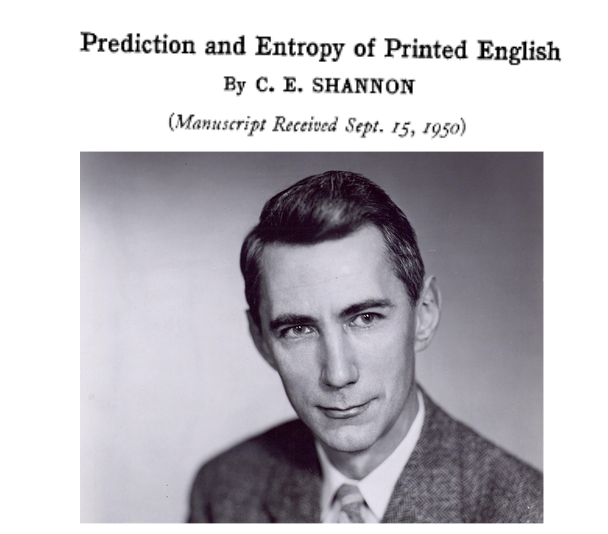
\includegraphics[scale = 0.4]{pics/shannon.png}
    \caption{Imagen de Shannon.}
    \label{fig:shannon}
\end{figure}

Por otro lado, en su libro \textit{Syntactic Structures} (1957), Noam Chomsky (en la Figura~\ref{fig:chomsky}), un lingüista y científico cognitivo, cuestionó la capacidad de los modelos de lenguaje probabilísticos para capturar y comprender la gramática del lenguaje humano \cite{chomsky2009syntactic}. Según Chomsky, la noción de ``gramaticamente correcto'' no puede ser equiparada a ``significativo'' en un sentido probabilista. Para ilustrar esto, presentó dos oraciones ficticias, ambas carentes de sentido:

\begin{enumerate}
    \item Colorless green ideas sleep furiously.
    \item Furiously sleep ideas green colorless.
\end{enumerate}

Aunque ambas oraciones carecen de significado, Chomsky argumentó que solo la primera se considera gramaticalmente correcta por los hablantes de inglés. Además, enfatizó que la corecctitud gramatical en inglés no puede determinarse únicamente mediante aproximaciones estadísticas. Aunque es poco probable que ninguna de las dos oraciones (1) o (2) haya surgido en documentos escritos en inglés, un modelo estadístico como los modelos de lenguaje vistos en este capítulo las consideraría igualmente ``remotas'' en relación al inglés. Sin embargo, la oración (1) es gramaticalmente correcta, mientras que la oración (2) no lo es, lo que destaca las limitaciones de los enfoques estadísticos para capturar la gramática. Estos argumentos retrasaron el estudio de los modelos de lenguaje probabilísticos durante varios años \cite{JurafskyBook}.

\begin{figure}[h]
    \centering
    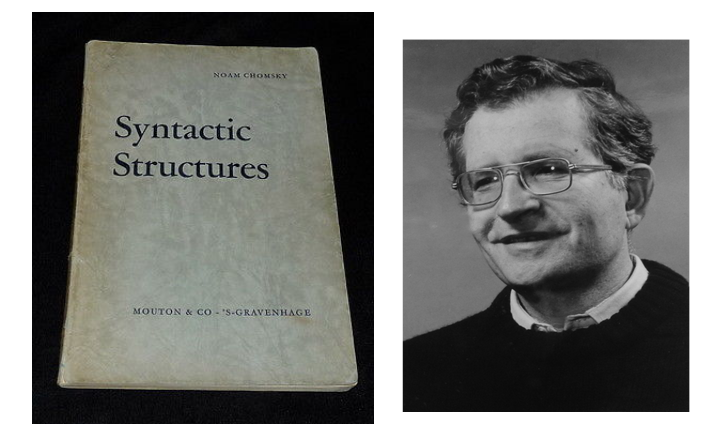
\includegraphics[scale = 0.4]{pics/chomsky.png}
    \caption{Imagen de Chomsky}
    \label{fig:chomsky}
\end{figure}


\section{Conclusiones}
La derivación de probabilidades en modelos de lenguaje probabilísticos implica tres pasos:
    \begin{enumerate}
        \item Expandir $p(w_1, w_2, \ldots, w_n)$ usando la regla de la Cadena.
        \item Aplicar los supuestos Independencia de Markov \\
        $p(w_i | w_1, w_2, \ldots, w_{i-2}, w_{i-1}) = p(w_i | w_{i-2}, w_{i-1})$.
        \item Suavizar las estimaciones utilizando conteos de orden inferior.
    \end{enumerate}
Otros métodos para mejorar los modelos de lenguaje incluyen introducir variables latentes para representar tópicos, conocidos como modelos de tópicos \cite{blei2003latent} presentados en el Capítulo~\ref{cap_ir}. O alternativamente, reemplazar $p(w_i | w_1, w_2, \ldots, w_{i-2}, w_{i-1})$ con una red neuronal predictiva y una ``capa de embedding'' para representar mejor contextos más grandes y aprovechar similitudes entre palabras en el contexto. \cite{bengio2000neural}

Los modelos de lenguaje modernos utilizan redes neuronales profundas en su estructura principal y tienen un vasto espacio de parámetros como se verá en el Capítulo~\ref{cap_llm}.

